\documentclass[a4paper,12pt,titlepage]{article}
\usepackage[utf8]{inputenc}
\usepackage{textcomp}
\usepackage{geometry}
\usepackage{fancyhdr}
\usepackage[yyyymmdd]{datetime}
\usepackage{tabularx}
\usepackage{parskip} 
\usepackage{longtable}
\usepackage{graphicx}
\usepackage{booktabs}
\pagestyle{fancy}
\lhead{Malcolm Vigren}
\rhead{D3.c}
\geometry{margin=3cm}
\renewcommand{\dateseparator}{--}
\renewcommand{\figurename}{Figur}

\begin{document}

\section*{Användarbarhetstest för Snowslide Car Edition}

\renewcommand*{\arraystretch}{1.4}
\begin{longtable}[l]{p{4cm} l}
    \textbf{Rapportdatum}    & \today \\
    \textbf{Testdatum   }    & 2017--03--01 \\
    \textbf{Utförd av   }    & Malcolm Vigren \\
    \textbf{Epost       }    & malvi108@student.liu.se \\
\end{longtable}

\subsection*{Sammanfattning}

Syftet med dessa användarbarhetstest är att testa hur användarvänlig en
prototyp för Snowslide Car Edition är. Det som uppgifterna som testades var
uppspelning av en spellista och skapande av ny användarprofil. Två personer
deltog i testet, och båda uppgifterna slutfördes av båda personerna. I den
andra uppgiften fann båda personerna vyn ointuitiv, och slutförde uppgiften
ineffektivt.

\subsection*{Metod}
\subsubsection*{Testpersoner}

2 personer testades. Personen som agerade som Pia var mycket representativ för
sin roll. Personen som spelade Tom var dock mindre representativ, då hon var en
kvinna i 20-års-åldern. Detta bedömdes dock vara acceptabelt, då Tom är
sekundär persona som är relativt datorvan, och en 90-talist borde ha ungefär
liknande nivå av datorvana.

\begin{longtable}[l]{c c c c}
    \textbf{Testperson} & \textbf{Persona som representerades} & \textbf{Ålder} & \textbf{Kön} \\ \midrule
    1 & Pia & 40--50 & Kvinna \\ \midrule
    2 & Tom & 18--25 & Kvinna \\ \midrule
\end{longtable}

\subsubsection*{Utförande}

Innan testet gjordes en introduktion, där det förklarades vad detta test skulle
gå ut på. I samband med detta fick deltagarna svara på frågor om deras
datorvana.

Testet startades sedan genom att prototypen startades utan förklaring om vad
vilken typ av produkt det var en prototyp av. Deltagarna blev tillfrågade om vad
de trodde att det var för produkt och vad det skulle användas till,
baserat på hur huvudmenyn ser ut. Efter detta fick deltagarna svaren på
frågorna, så att de förstod vad prototypen var innan de började. Efter detta
fick deltagarna börja utföra uppgifterna, under uppmaningen att tänka högt.

Uppgifterna som användarna skulle utföra var nedskrivna på lappar. Den första
uppgiften var likadan för båda deltagarna, som gick ut att spela upp en
spellista. I den andra uppgiften skulle en användarprofil ställas in, den ena
personen fick ställa in en barnprofil för ett barn (för personan Pia), och den
andra fick ställa in en profil utan föräldrarprivilegier (för personan Tom).

Efter testet ställdes utvärderande frågor om deltagarnas upplevelse.

\subsubsection*{Data som insamlades}

Förutom svaren på frågorna så antecknades huruvida varje testperson klarade
uppgifterna, om användaren försökte ta andra vägar än de som var tänkta,
eventuella frustrationer de visade samt övriga problem som användarna hade.

\subsection*{Större fynd och rekommendationer}

De största problemen som upptäcktes:

\begin{itemize}
    \item Fliksystemet för profilinmatning var otydlig.
    \item Otydligt hur en profil skulle sparas.
\end{itemize}

Det användarna båda hade problem med var vyn för att skapa profiler. När de
skulle fylla i mer information än bara namnet så trodde båda att man skulle
trycka på "Klar" för att komma till nästa uppgifter, där det i själva verket
fanns ett fliksystem för olika typer av information, och att "Klar" sparade
profilen som skapades. Båda tyckte med andra ord att det var otydligt hur man
matade in olika typer av information och sedan sparade.

En lösning till detta problem vore att göra om texten på "Klar"-knappen till
"Spara", och att ha alla alternativ för profilen som en scrollvy med
undermenyer, för att göra det tydligt att man kan ställa in mer än bara namnet.

Vid den första uppgiften trodde båda testpersonerna att det var meningen att
musiken skulle spelas i Spotify, istället för musik-appen, men det är nog inget
problem med designen så mycket som ett problem med uppgiftsinstruktionen.

\newpage
\subsection*{Detaljerade fynd och rekommendationer}

\subsubsection*{Inledande frågor innan testet}

Dessa frågor ställdes innan respektive testtillfälle påbörjades:

\begin{longtable}[c]{ >\raggedright p{5cm} p{4.7cm} p{4.7cm} }
    \textbf{Fråga} & \textbf{Svar person 1} & \textbf{Svar person 2} \\
    \midrule
    Är du van vid att använda datorer? & Ja & Ja \\ \midrule
    Är du van vid att använda pekskärmsbaserade enheter? & Ja & Ja \\ \midrule
    Har du lätt för att lära dig hur man använder nya appar? & Tror det & Ja
    (tveksamt) \\ \midrule
\end{longtable}

\subsubsection*{Inledande frågor under testet}

Dessa frågor ställdes när prototypens huvudmeny startats innan testpersonerna
påbörjat sina uppgifter, för att fånga initiala intryck. Detta markerar start
av testet.

\begin{longtable}[c]{ >\raggedright p{5cm} p{4.7cm} p{4.7cm} }
    \textbf{Fråga} & \textbf{Svar person 1} & \textbf{Svar person 2} \\
    \midrule
    Vad tror du denna är för typ av applikation? & En iPad eller PC & Ett
    mediaprogram, som en telefon med mappstruktur. \\ \midrule
    Var tror denna produkt är tänkt att användas? & Privat bruk på fritiden. &
    I en telefon. \\ \midrule
    Vilka tror du målgruppen är? & Yrkesfolk, datorvana personer mellan 20-60,
    även tonåringar. & De som använder gamla telefoner, alltså de som inte är
    teknikvana. \\ \midrule
    Vad tror du man kan göra med denna applikation? & Profilering, nå appar. &
    Spotify, Netflix, spel mm. \\ \midrule
\end{longtable}

\newpage
\subsubsection*{Uppgift 1 - Spela musik}

\textit{%
Du är sugen på att lyssna på musik. Spela upp din spellista "Mina favoriter" så
att låtarna blandas.
}

Båda testpersonerna deltog i detta test, och båda klarade av uppgiften. Båda
testpersonerna försökte öppna Spotify-appen innan de insåg att "Min
Musik"-appen skulle användas, men använde sedan den tänkta vägen för att spela
upp den angivna spellistan.

\subsubsection*{Uppgift 2.1 - Skapa ny profil (anpassad för föräldrar)}

\textit{%
Du ska precis åka på bilresa och sitter i framsätet. När systemet startar möts
du av vyn framför dig, och systemet saknar en profil för ditt barn Lisa som
sitter där bak till höger. Skapa en användarprofil för Lisa, med namnet "Lisa",
blå profilbild. Gör vidare så att profilen blir en barnprofil, där maximala
tillåtna åldersgränsen är 9 år, får max spela spel 4 timmar per dag, får titta
på film max 4 timmar per dag, och får inte köpa saker i affären.
}

Testperson 1 gjorde detta test, och klarade uppgiften, dock inte utan problem.
Först fylldes namnet i, och sedan trycktes "Klar"-knappen innan resten av
informationen var ifylld. Uppgiften startades därför om, eftersom prototypen
inte kontrollerade om det var rätt ifyllt. Nu insåg testpersonen hur
informationen är tänkt att fyllas i, så uppgiften slutfördes korrekt på detta
försök.

Under uppgiften uttryckte personen frustration över hur det inte fanns en
"Spara"-knapp, och att det var otydligt hur man fyllde i resten av
informationen. En rekommendation som man kan ta från detta är att ändra texten
från "Klar"-knappen till "Spara", samt att ha alternativen i en hierarkisk
scrollmeny istället för ett fliksystem.

\subsubsection*{Uppgift 2.2 - Skapa ny profil (anpassad för barn)}

\textit{%
Du vill skapa en ny profil för din syster Lisa. Skapa därför en profil som
heter "Lisa", med blå profilbild.
}

Testperson 2 gjorde detta test, och klarade uppgiften, dock återigen inte
felfritt. Personen öppnade först musik-appen, innan hon insåg att det var "Byt
Profil"-knappen som skulle användas. Hon matade in namnet, men tryckte precis
som testperson 1 på "Klar" för tidigt, men hon gick in igen och satte
profilbilden korrekt.

Precis som i uppgift 2.1 så tyckte personen att det var otydligt att det var
ett fliksystem, och att det såg ut som "Klar" skulle leda till profilbilden.
Rekommendationen för detta är samma som för 2.1, då det är samma problem.

\subsubsection*{Avslutande frågor}

Dessa frågor ställdes efter testpersonerna utfört sina uppgifter.

\begin{longtable}[c]{>\raggedright p{5cm} >\raggedright p{4.7cm} p{4.7cm} }
    \textbf{Fråga} & \textbf{Svar person 1} & \textbf{Svar person 2} \\ \midrule
    Var det enkelt? & Ganska enkelt & Inte den andra uppgiften \\ \midrule
    Vad tyckte du var bra? & Enkelt och snabbt att hitta saker & Enkelt att
    välja musik \\ \midrule
    Vad tyckte du var mindre bra? & Saknade "Slutför"-knapp i uppgift 2.1 & "Ny Profil" var ologisk. \\ \midrule
    Vad kan förbättras? & Tydligare bekräftelse av handlingar. & Vet inte. \\ \midrule
    Övriga kommentarer? & Inga & Använd vita element istället för gråa.
\end{longtable}

\newpage

\section*{Bilaga - skärmbilder}

\begin{figure}[h]
    \centering
    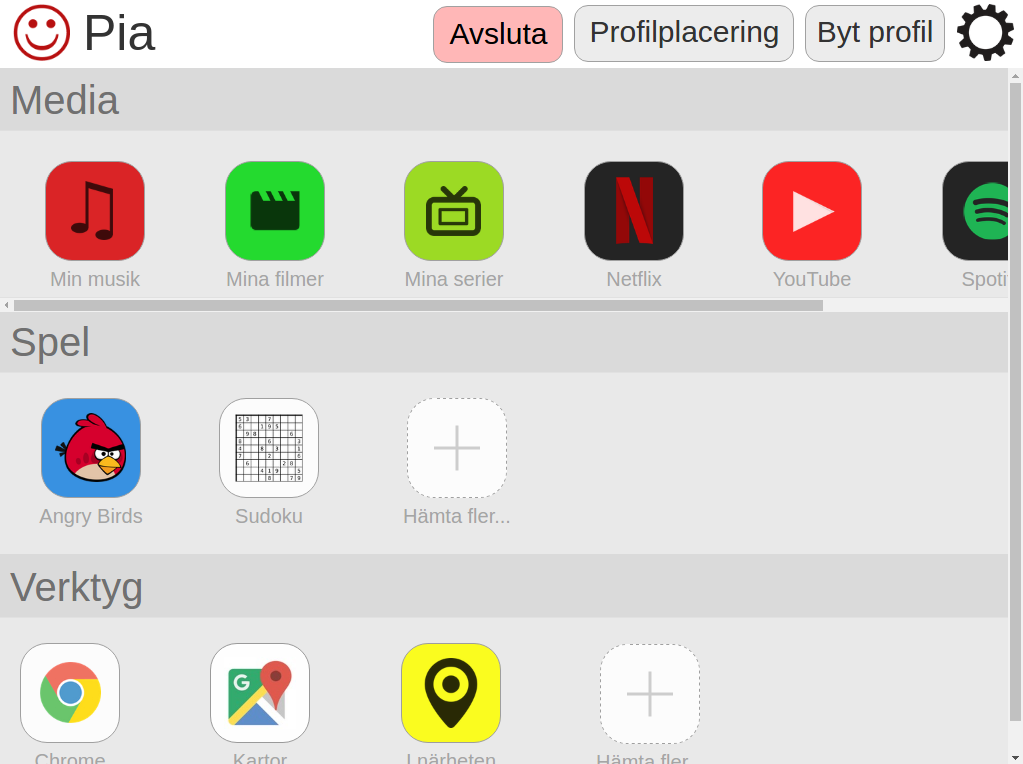
\includegraphics[width=10cm]{../screenshots/main_menu_pia.png}
    \caption{Huvudmenyn för föräldrar}
\end{figure}

\begin{figure}[h]
    \centering
    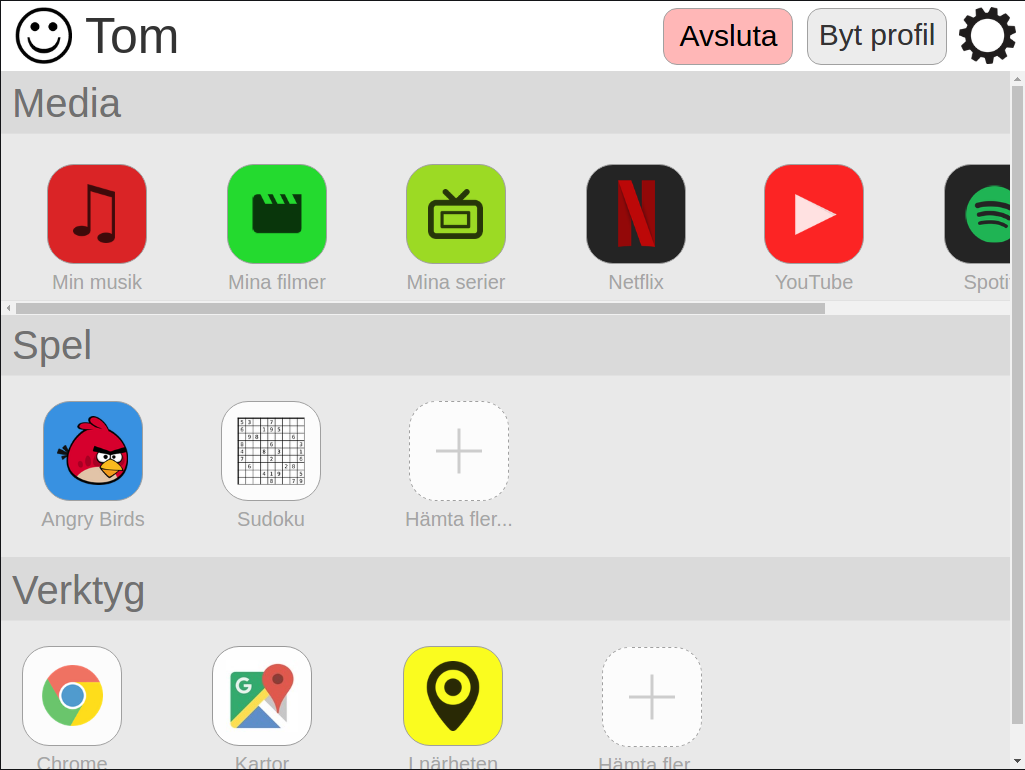
\includegraphics[width=10cm]{../screenshots/main_menu_tom.png}
    \caption{Huvudmenyn för barn, saknar "Profilplacering"-knapp}
\end{figure}

\begin{figure}[h]
    \centering
    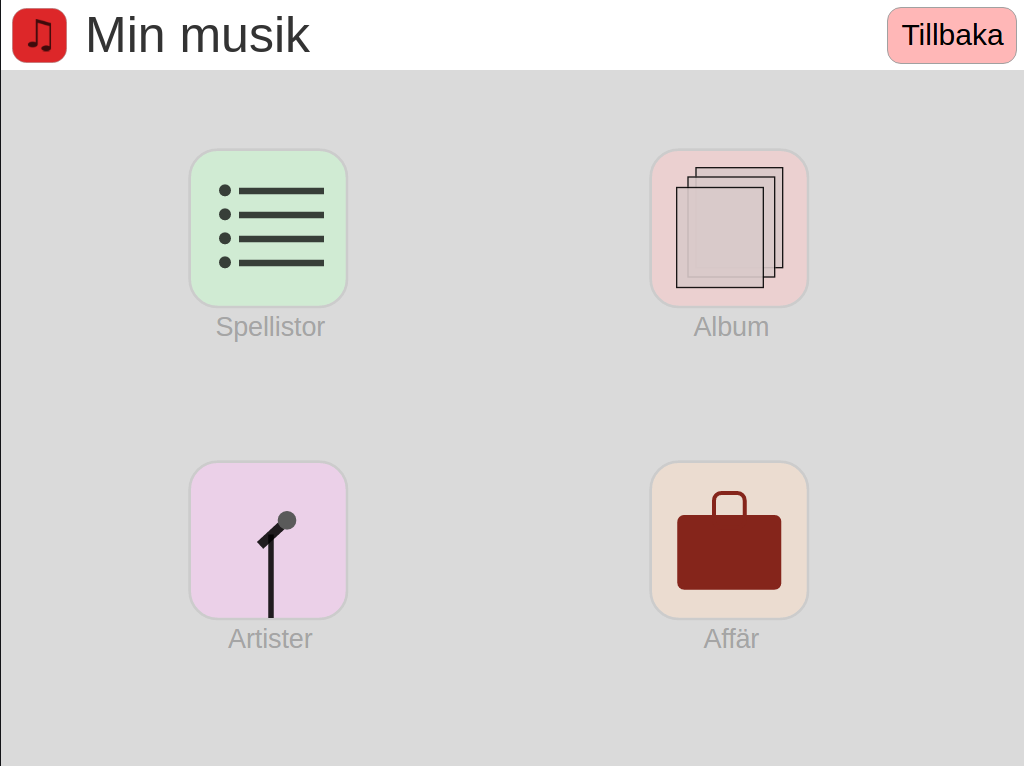
\includegraphics[width=10cm]{../screenshots/music.png}
    \caption{Menyn i Musik-appen}
\end{figure}

\begin{figure}[h]
    \centering
    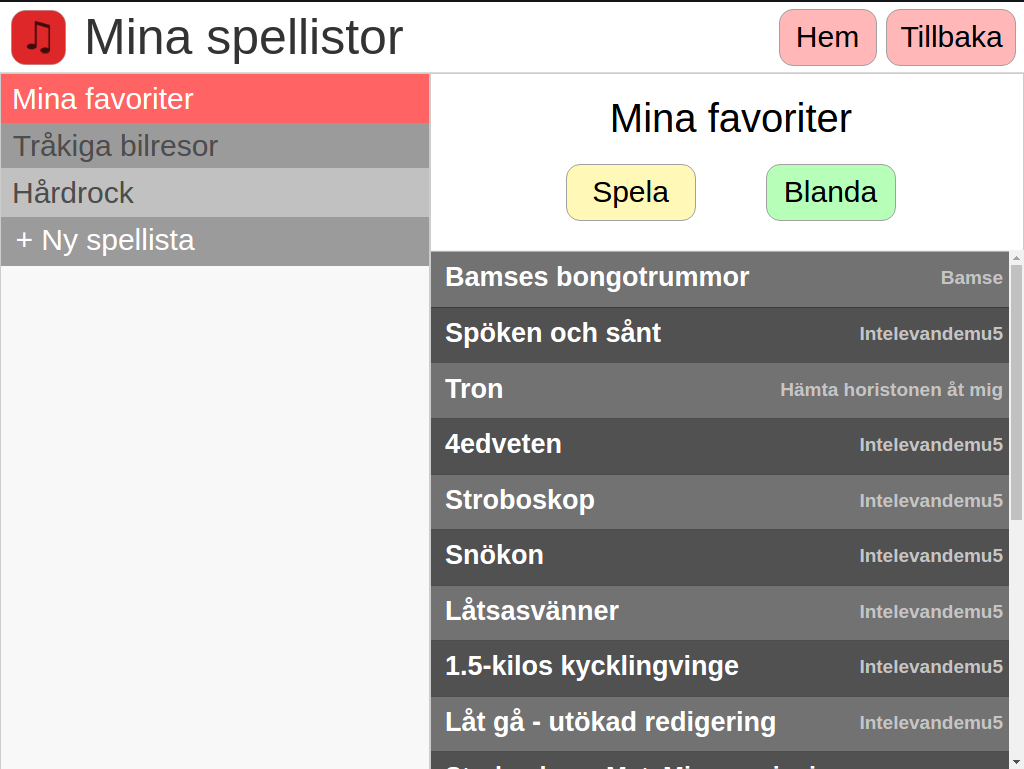
\includegraphics[width=10cm]{../screenshots/playlists.png}
    \caption{Vyn för spellistor i musik-appen}
\end{figure}

\begin{figure}[h]
    \centering
    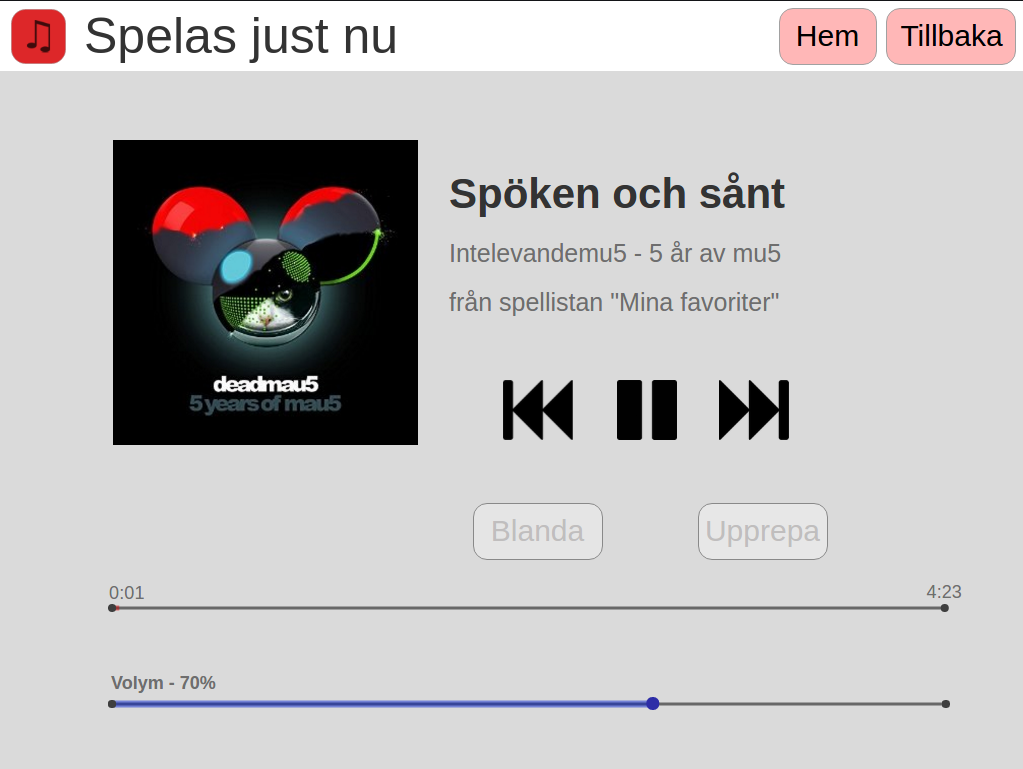
\includegraphics[width=10cm]{../screenshots/player.png}
    \caption{Spelningsvyn i musik-appen}
\end{figure}

\begin{figure}[h]
    \centering
    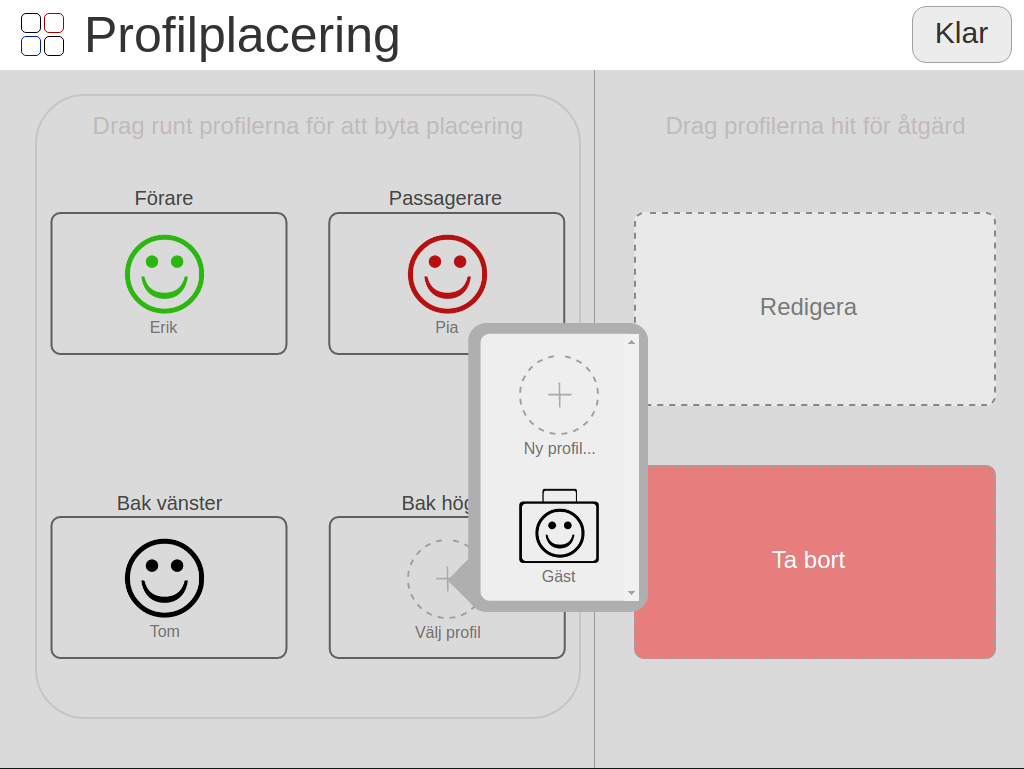
\includegraphics[width=10cm]{../screenshots/profile_placement.png}
    \caption{Profilplaceringsvyn, endast föräldrar har åtkomst till denna}
\end{figure}

\begin{figure}[h]
    \centering
    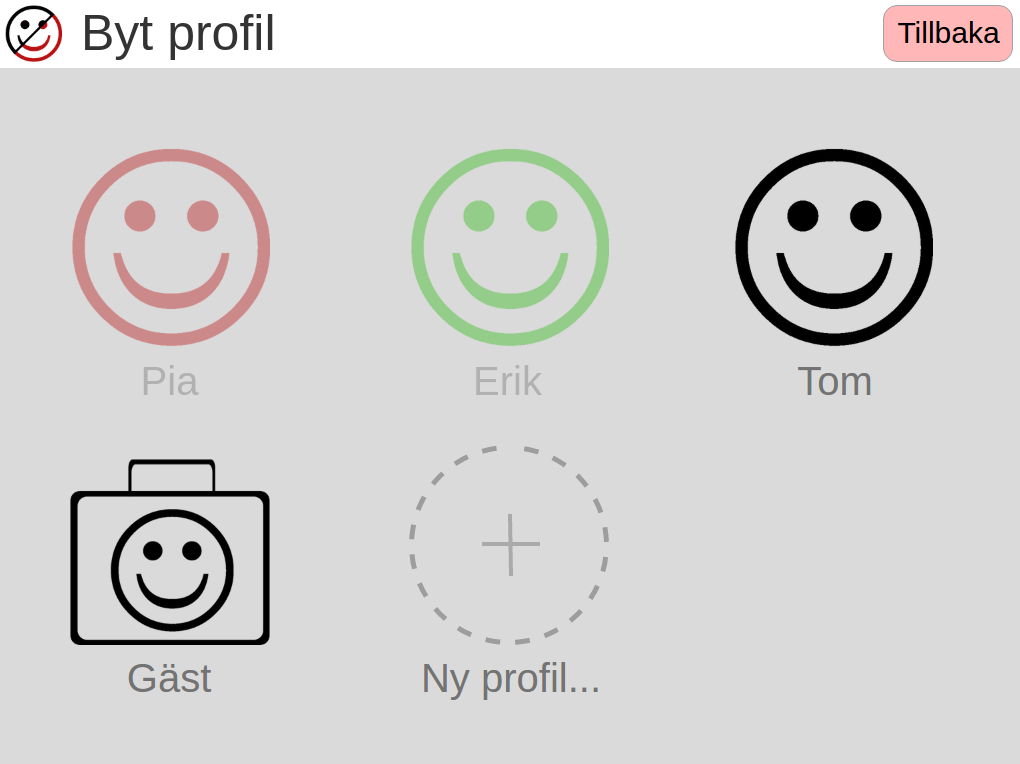
\includegraphics[width=10cm]{../screenshots/switch_profile.png}
    \caption{Byt-profil-vyn, Pia och Erik kan inte väljas eftersom Tom är
    inloggad}
\end{figure}

\begin{figure}[h]
    \centering
    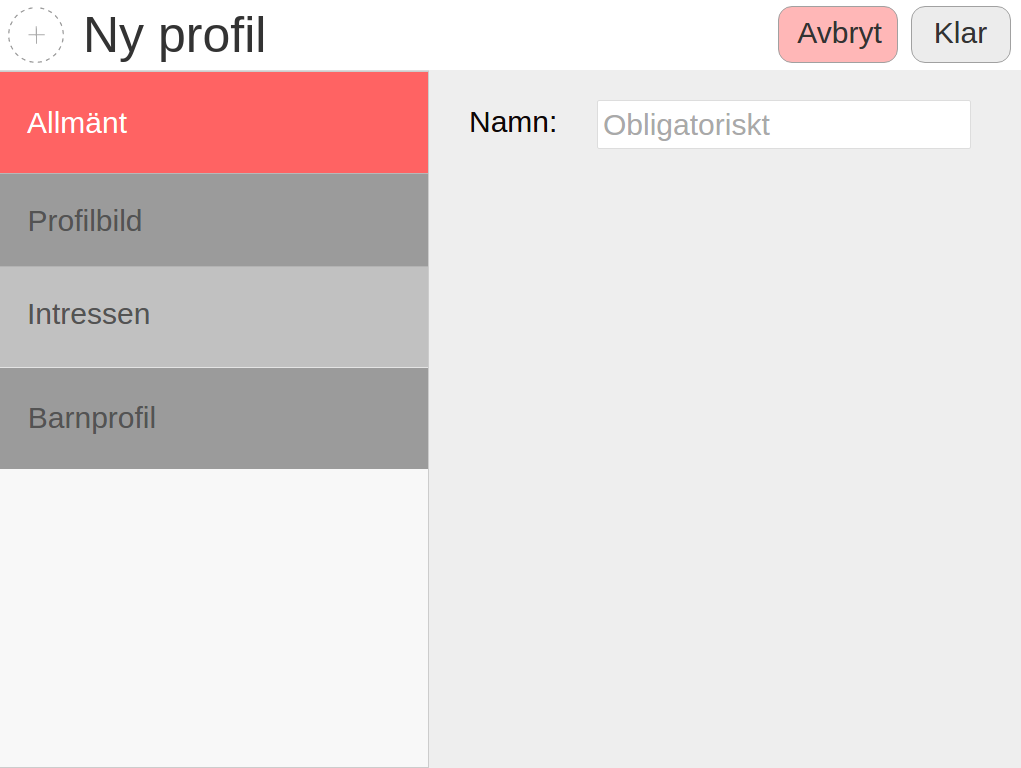
\includegraphics[width=10cm]{../screenshots/new_profile_general.png}
    \caption{Ny-profil-vyn, i "Allmänt"-fliken}
\end{figure}

\begin{figure}[h]
    \centering
    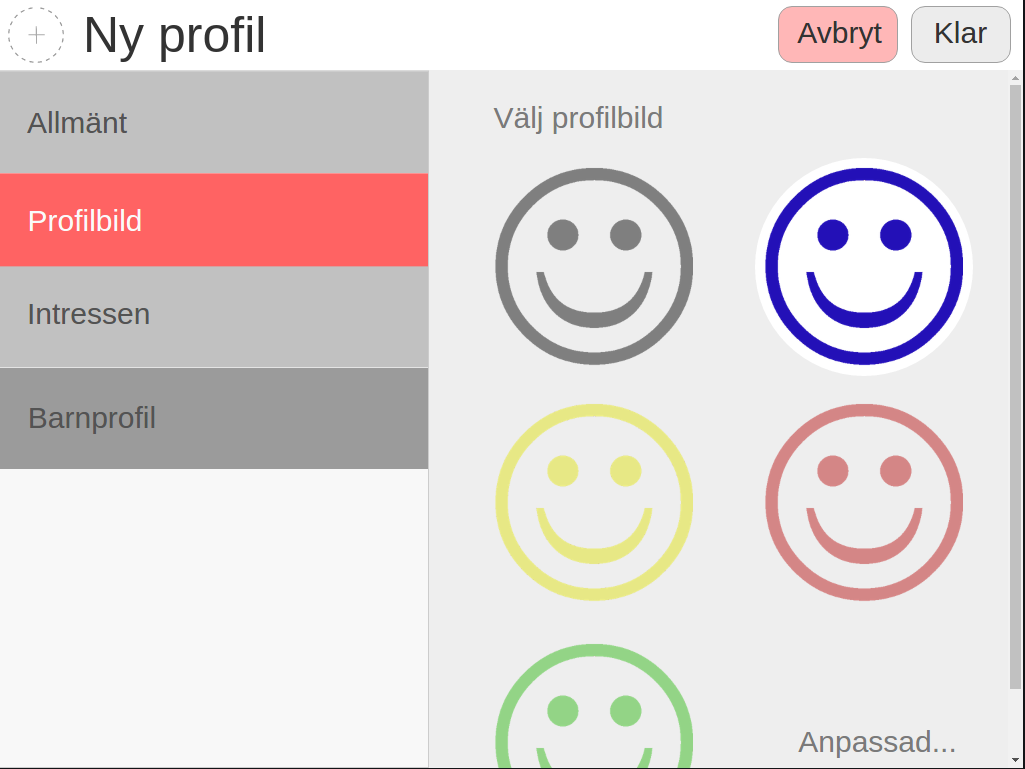
\includegraphics[width=10cm]{../screenshots/new_profile_pic.png}
    \caption{Ny-profil-vyn, i "Profilbild"-fliken}
\end{figure}

\begin{figure}[h]
    \centering
    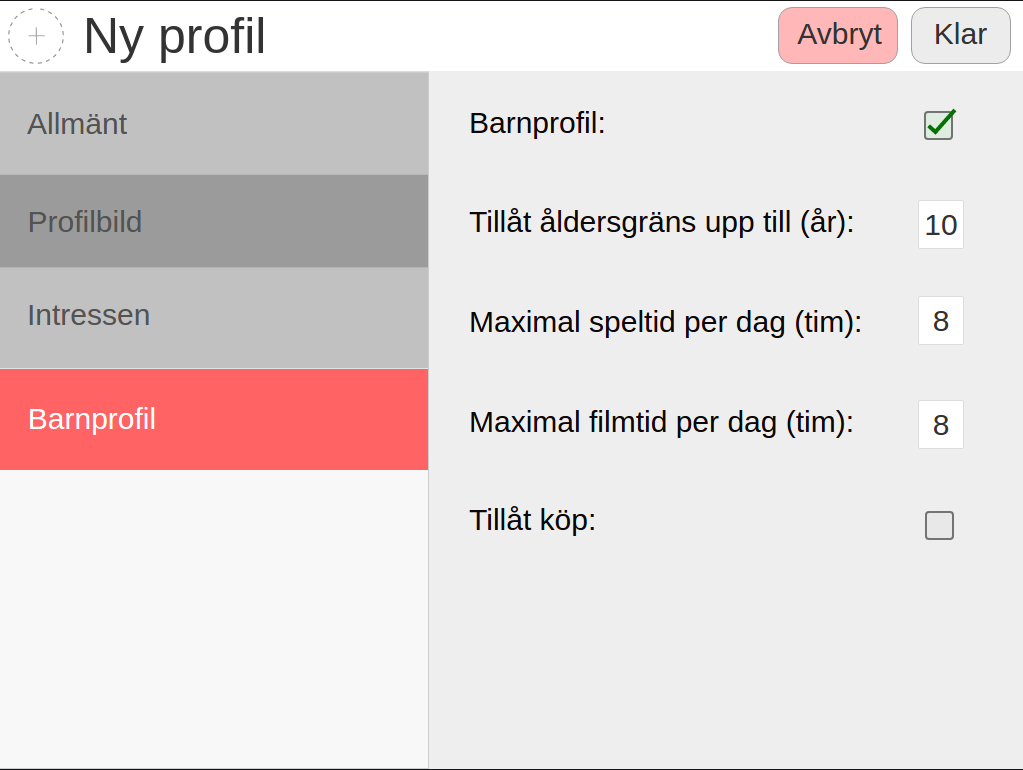
\includegraphics[width=10cm]{../screenshots/new_profile_kids.png}
    \caption{Ny-profil-vyn, i "Barnprofil"-fliken}
\end{figure}

\begin{figure}[h]
    \centering
    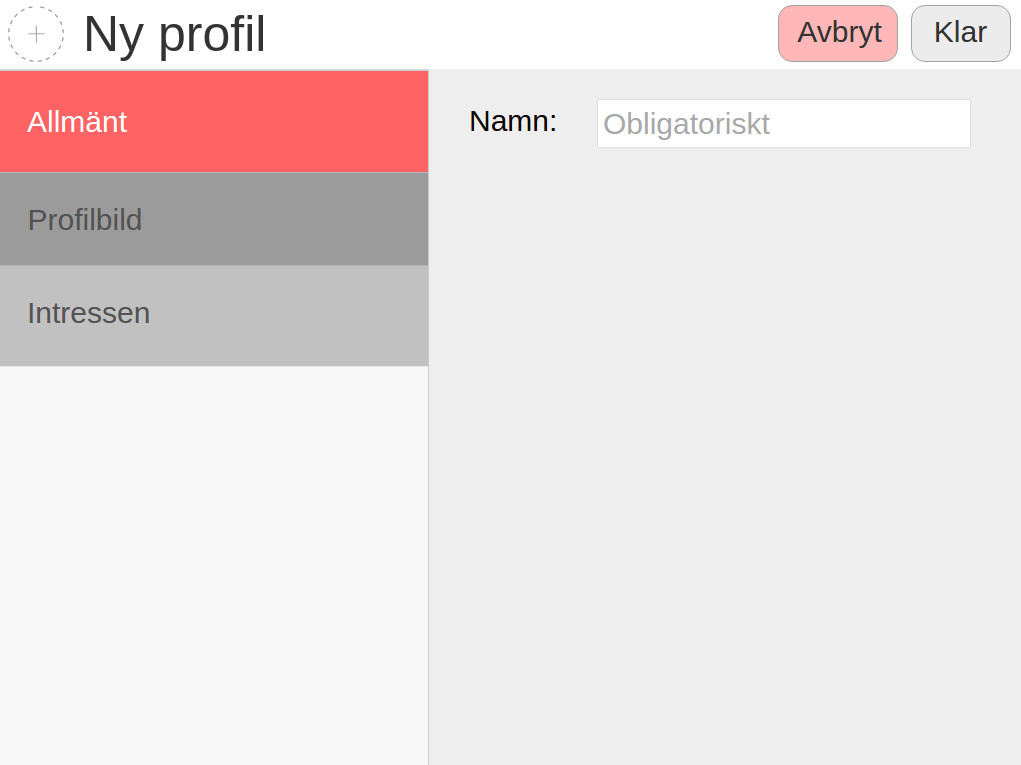
\includegraphics[width=10cm]{../screenshots/new_profile_no_kids.png}
    \caption{Ny-profil-vyn, utan "Barnprofil"-fliken då användaren är ett barn}
\end{figure}

\end{document}
